\documentclass[a4paper]{article}
\linespread{1.6}
\usepackage{geometry}
\usepackage{setspace}
\usepackage{amsmath}
\usepackage{amssymb}
\usepackage[pdftex]{graphicx}
\usepackage{float}
\usepackage{subfigure}
\usepackage{listings}
\geometry{left=1.5cm,right=1.5cm,top=2.5cm,bottom=2.5cm}

\begin{document}
\begin{spacing}{2.0}
\begin{flushleft}\begin{huge}EEL5840 Fundamental Machine Learning   Homework 1\end{huge}\end{flushleft}
\begin{flushright}\begin{Large} Hudanyun Sheng \end{Large}\end{flushright}

\huge\textbf{ Question 1}      \Large{Solution:} \\
	\normalsize 
	MATLAB code is shown below: 
	\begin{lstlisting}
upBound = 1; %set the upper bound for the training data
lowBound = 0; %set the lower bound for the training data
num = 100; % # of desired training data
step = (upBound - lowBound)/(num-1);
x_train = lowBound+step/2:step:upBound+step/2;
x_test = lowBound+step/2+0.1:step:upBound+step/2+0.1;
mu = 0;
sigma = 0.1;
e_train = normrnd(mu, sigma, [1, num]);
e_test = normrnd(mu, sigma, [1, num]);
t = (sin(2*pi*x_train) + e_train)'; % labels of the train data
t_test = (sin(2*pi*x_test) + e_test)';
max_M = 10;
ERMS_train = zeros(1, max_M+1);
ERMS_test = zeros(1, max_M+1);
for M = 0:max_M
    X = (x_train'.^ (0:1:M));
    X_test = (x_test'.^ (0:1:M));
    w = ((X'*X)\X')*t;
    y1 = sin(2*pi*x_train); % the true value of the sine function
    y2 = t'; % the true label of training data (sine function with error)
    y3 = (X*w)'; % the fitted polynomial
    y4 = (X_test*w)'; % the predicted value of test data
    y5 = t_test'; % the label of test set
    figure
    plot(x_train,y1', 'Linewidth', 3);
    hold on
    scatter(x_train,y2);
    hold on
    plot(x_train,y3, 'Linewidth', 3);
    title(['Training Data and Estimated Polynomial when M=' num2str(M)])
    legend('True Sine Function','Training Data', 'Estimated Polynomial')
    xlabel('x')
    ylabel('t')
    print(gcf,'-djpeg',[num2str(M),'train.jpeg']);
    hold off    
    figure
    plot(x_test,y4, 'Linewidth', 3);
    hold on
    scatter(x_test, y5)
    title(['Test Data and Predicted Value when M=' num2str(M)])
    legend('Test Data', 'Predicted value of test')
    xlabel('x')
    ylabel('t')
    print(gcf,'-djpeg',[num2str(M),'test.jpeg']);
    hold off
    ERMS_train(M+1) = sqrt(mean((y2 - y3).^2));
    ERMS_test(M+1) = sqrt(mean((y4 - y5).^2));
end
figure(101)
plot(0:1:max_M, ERMS_train, 'o-', 'Linewidth', 3)
hold on
plot(0:1:max_M, ERMS_test, 'o-', 'Linewidth', 3)
legend('train', 'test')
xlabel('M')
ylabel('E_{RMS}')
print(gcf,'-djpeg','ERMS.jpeg');
hold off
	\end{lstlisting}
	I generated 100 training data from the range $[0, 1]$, based on the sine curve, with selected step size, and added zero-mean Gaussian noise to the training set. I generated the test data set in the same way, while the range changed to $[0.1, 1.1]$. And I changed the order of the model from 0 to 10, the selected results are shown below: 
	\begin{figure}[H]
	    \begin{minipage}[t]{0.5\textwidth}
	        \centering
	        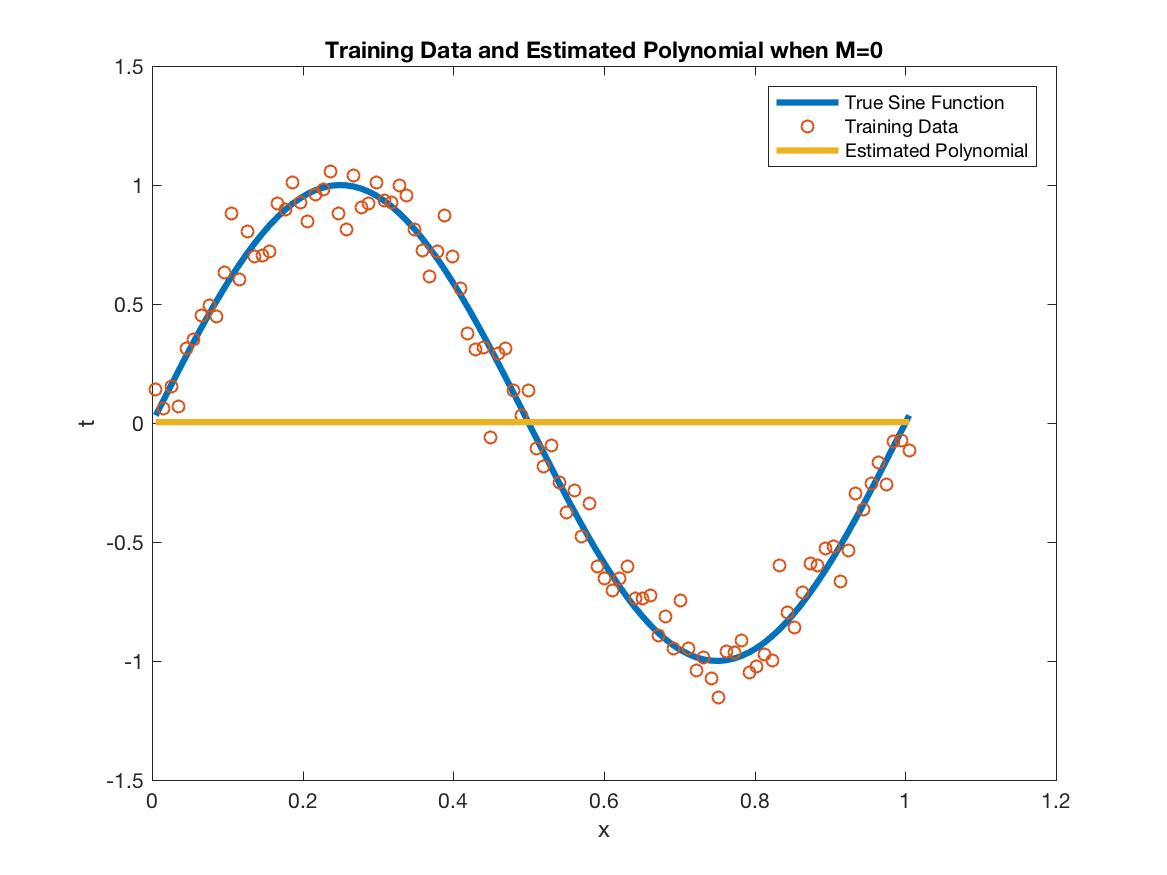
\includegraphics[width=3.4in]{0train.jpeg}
	        \caption{Training: M = 0}
	        \label{fig:side:a}
	    \end{minipage}%
	  \begin{minipage}[t]{0.5\textwidth}
	      \centering
	      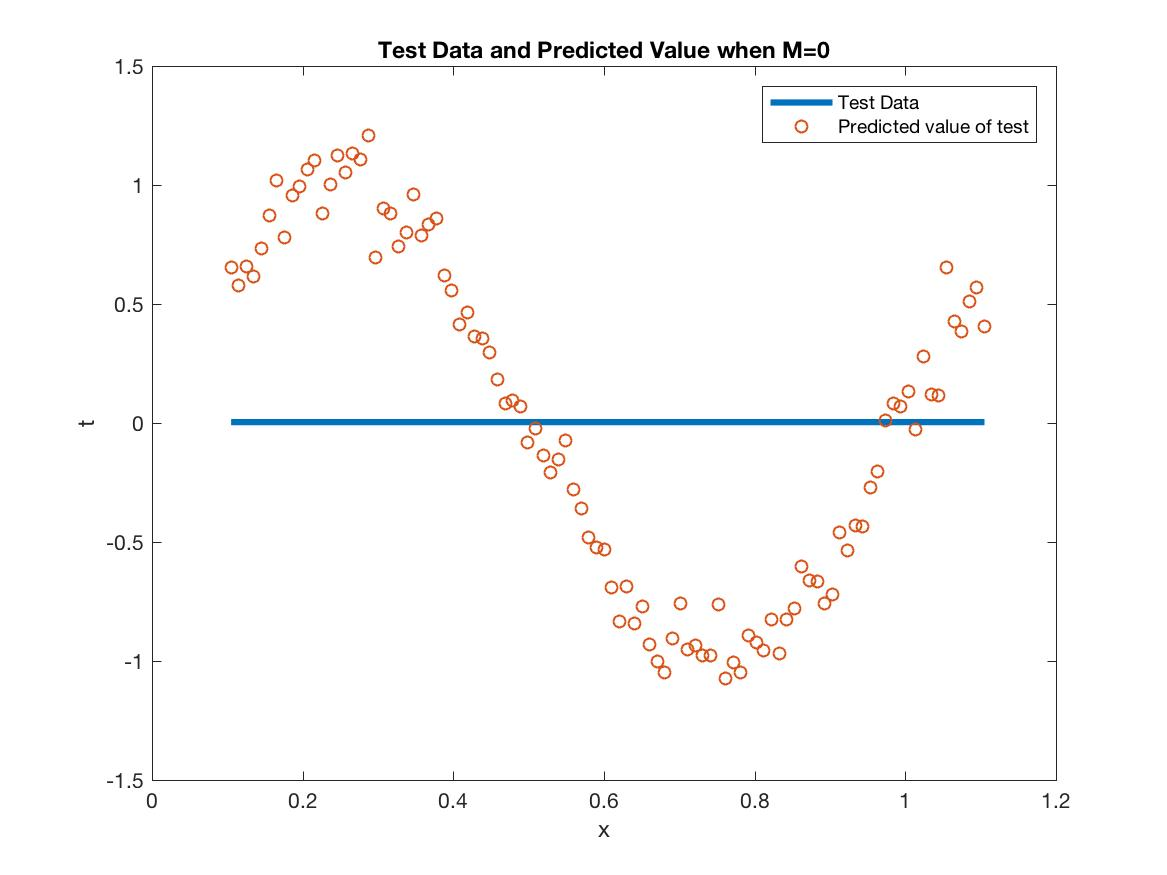
\includegraphics[width=3.4in]{0test.jpeg}
	      \caption{Test: M = 0}
	      \label{fig:side:b}
	    \end{minipage}
	\end{figure}
	
	\begin{figure}[H]
	    \begin{minipage}[t]{0.5\textwidth}
	        \centering
	        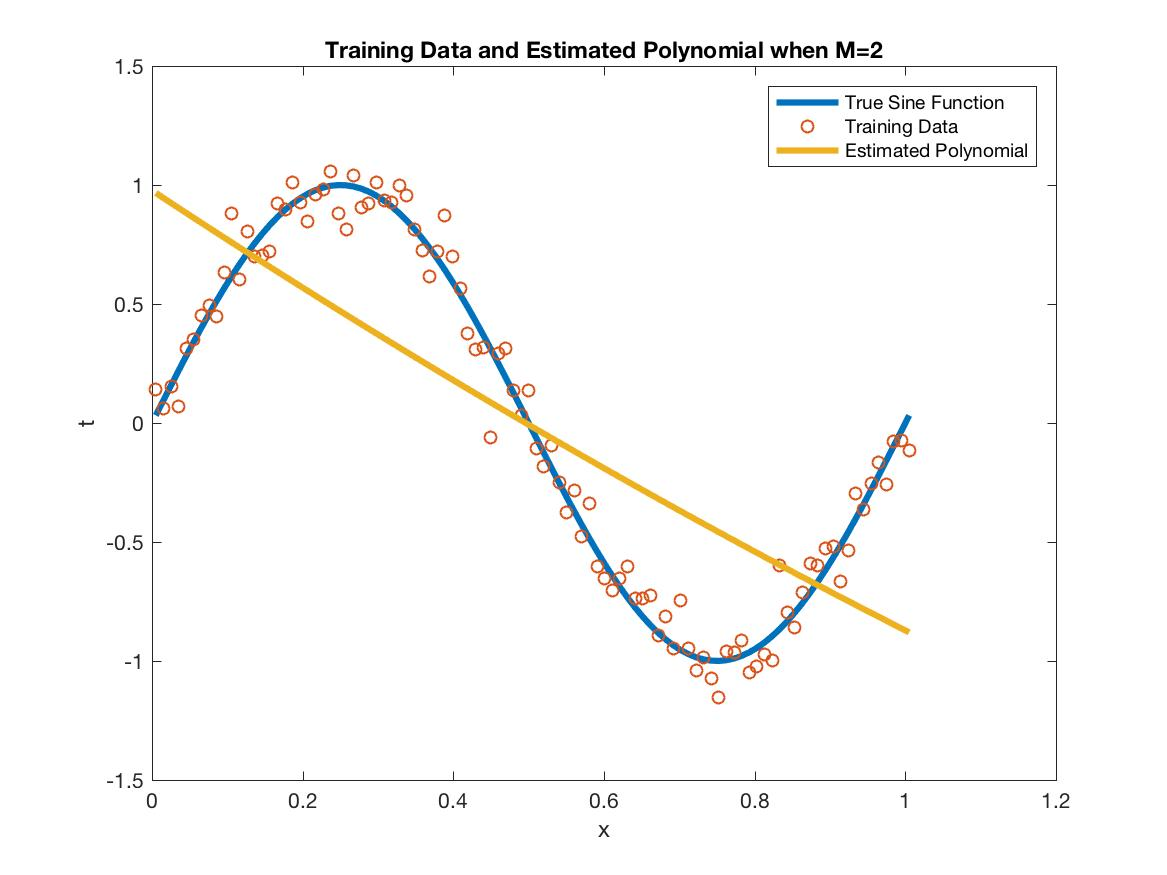
\includegraphics[width=3.4in]{2train.jpeg}
	        \caption{Training: M = 2}
	        \label{fig:side:a}
	    \end{minipage}%
	  \begin{minipage}[t]{0.5\textwidth}
	      \centering
	      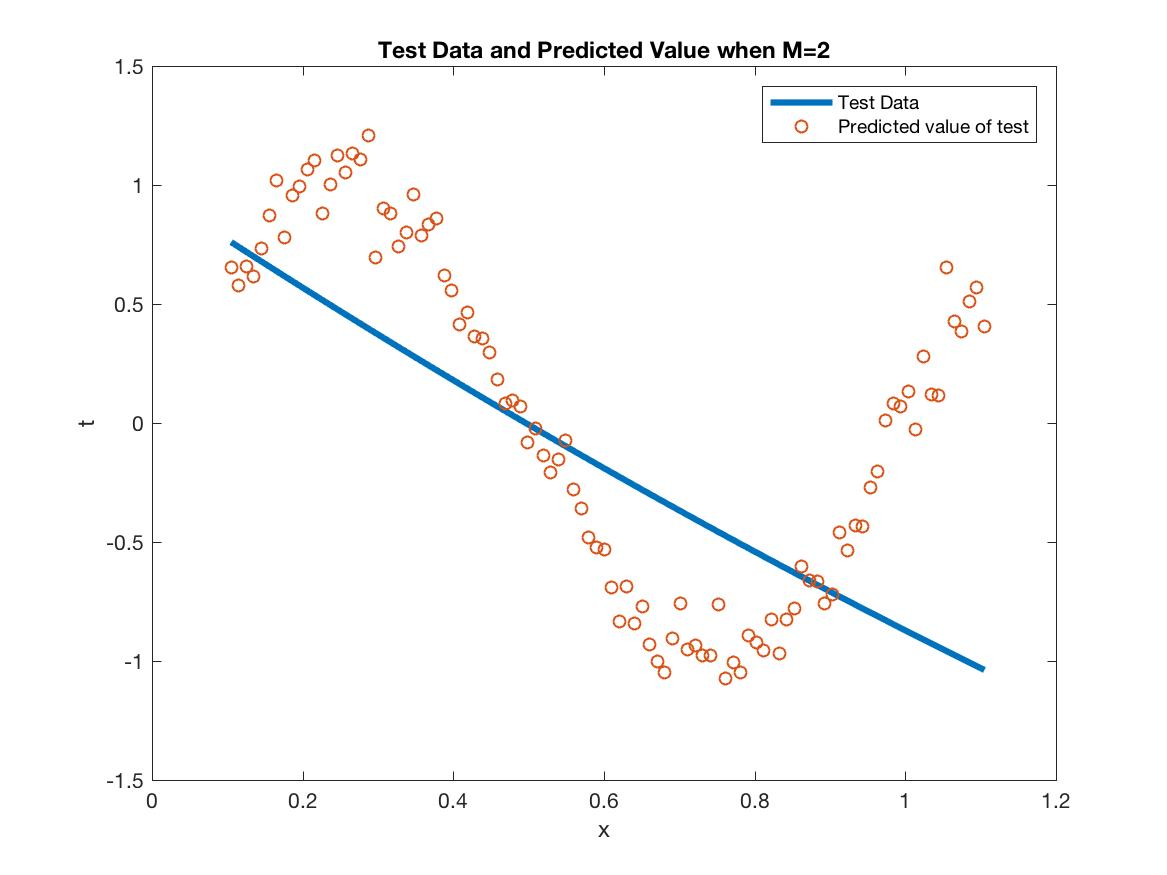
\includegraphics[width=3.4in]{2test.jpeg}
	      \caption{Test: M = 2}
	      \label{fig:side:b}
	    \end{minipage}
	\end{figure}
	
	\begin{figure}[H]
	    \begin{minipage}[t]{0.5\textwidth}
	        \centering
	        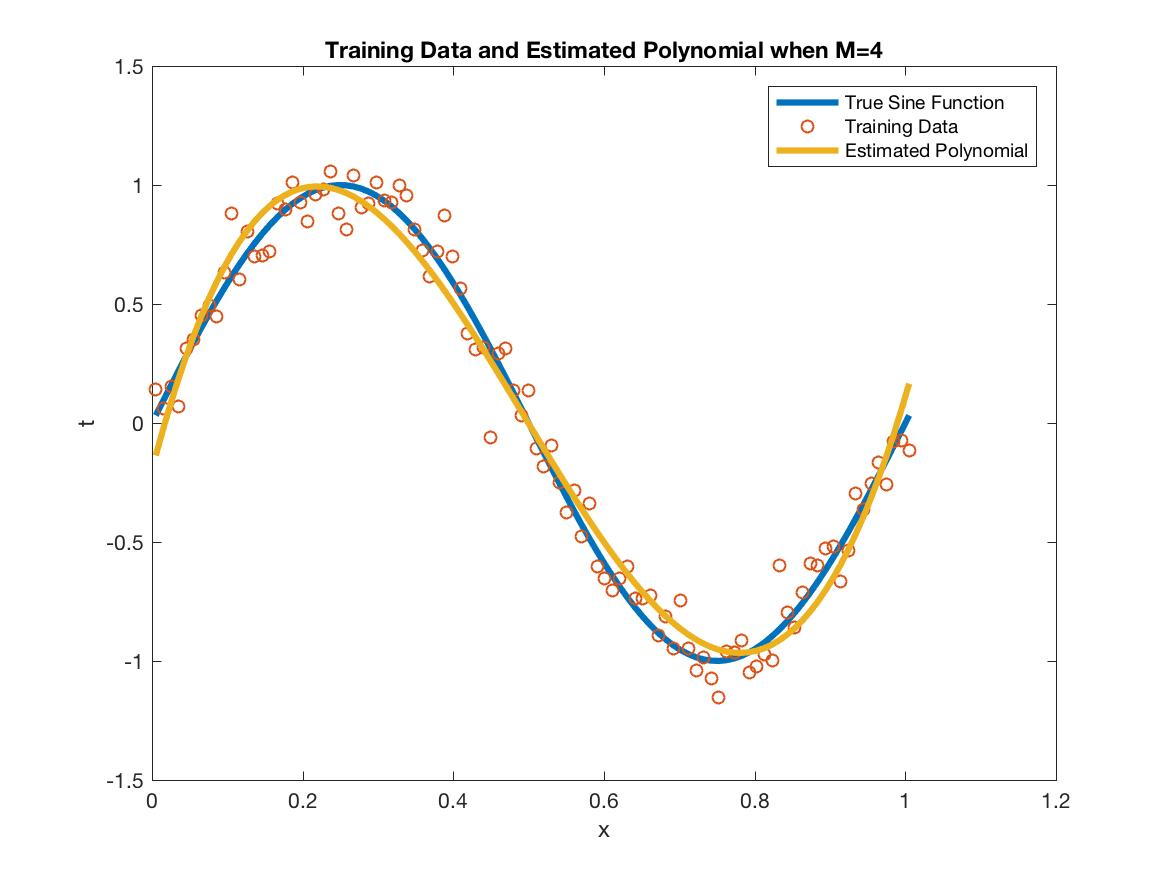
\includegraphics[width=3.4in]{4train.jpeg}
	        \caption{Training: M = 4}
	        \label{fig:side:a}
	    \end{minipage}
	  \begin{minipage}[t]{0.5\textwidth}
	      \centering
	      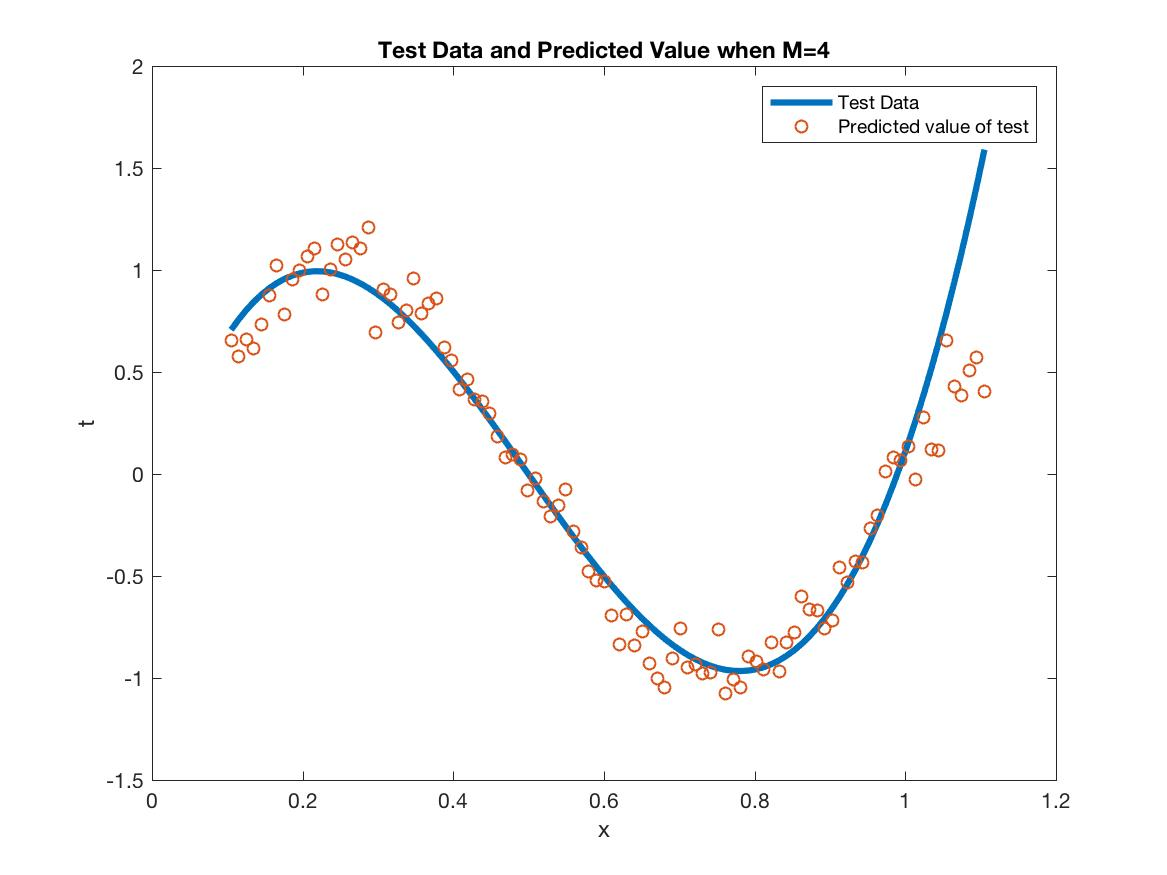
\includegraphics[width=3.4in]{4test.jpeg}
	      \caption{Test: M = 4}
	      \label{fig:side:b}
	    \end{minipage}
	\end{figure}	
	
		\begin{figure}[H]
	    \begin{minipage}[t]{0.5\textwidth}
	        \centering
	        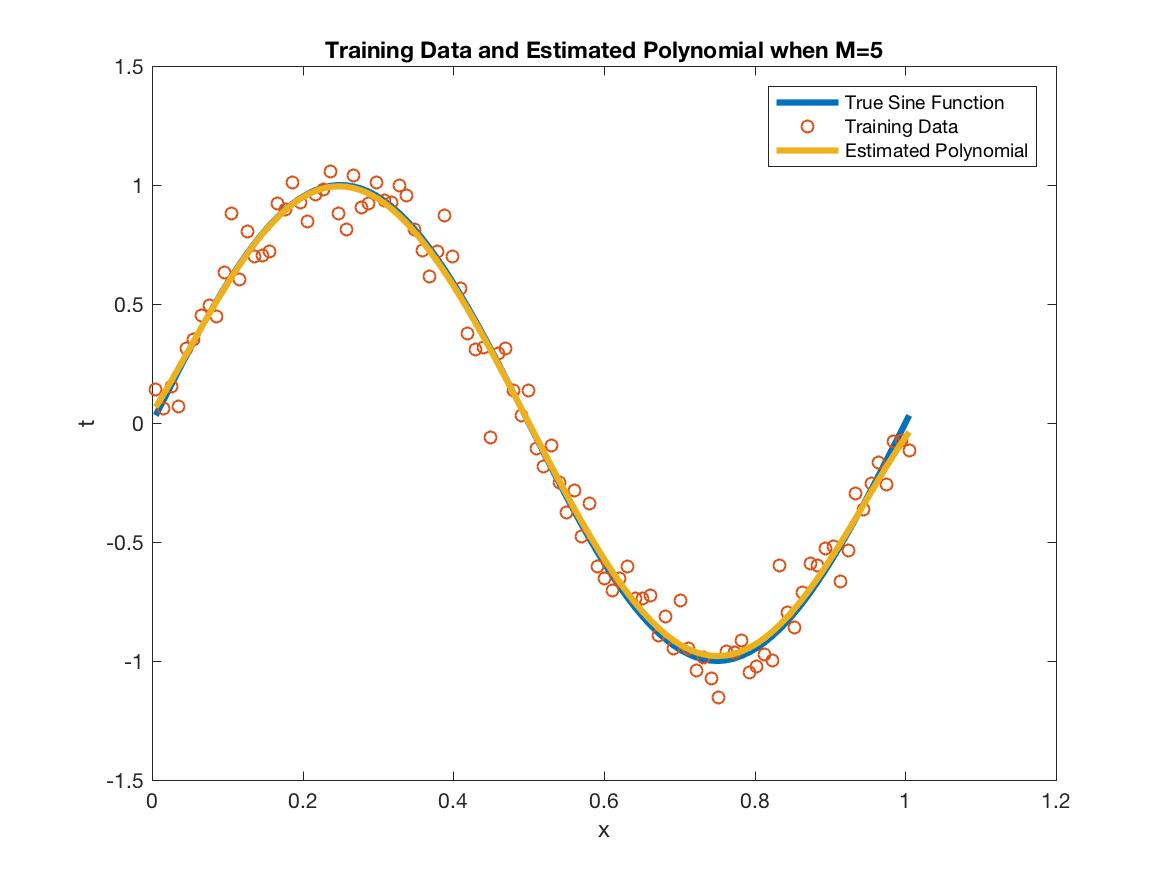
\includegraphics[width=3.4in]{5train.jpeg}
	        \caption{Training: M = 5}
	        \label{fig:side:a}
	    \end{minipage}
	  \begin{minipage}[t]{0.5\textwidth}
	      \centering
	      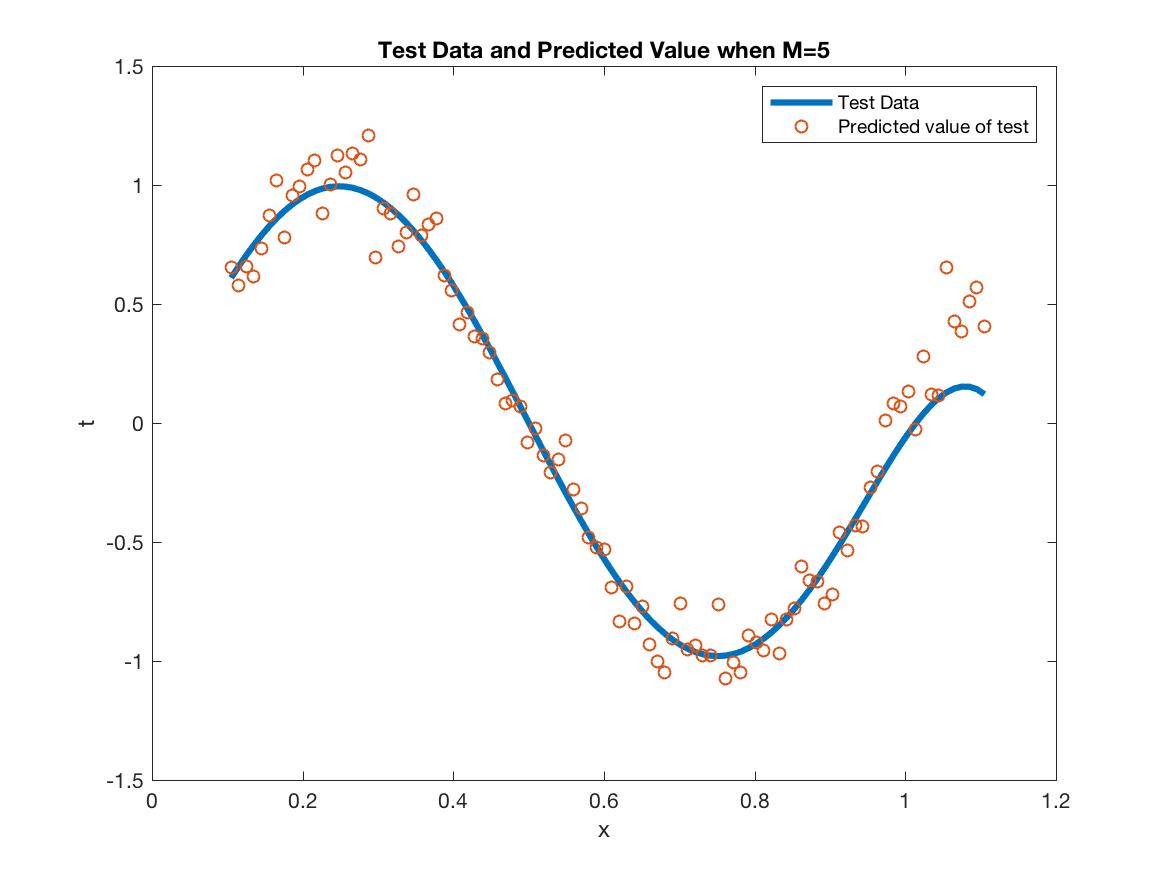
\includegraphics[width=3.4in]{5test.jpeg}
	      \caption{Test: M = 5}
	      \label{fig:side:b}
	    \end{minipage}
	\end{figure}	
	
	\begin{figure}[H]
	    \begin{minipage}[t]{0.5\textwidth}
	        \centering
	        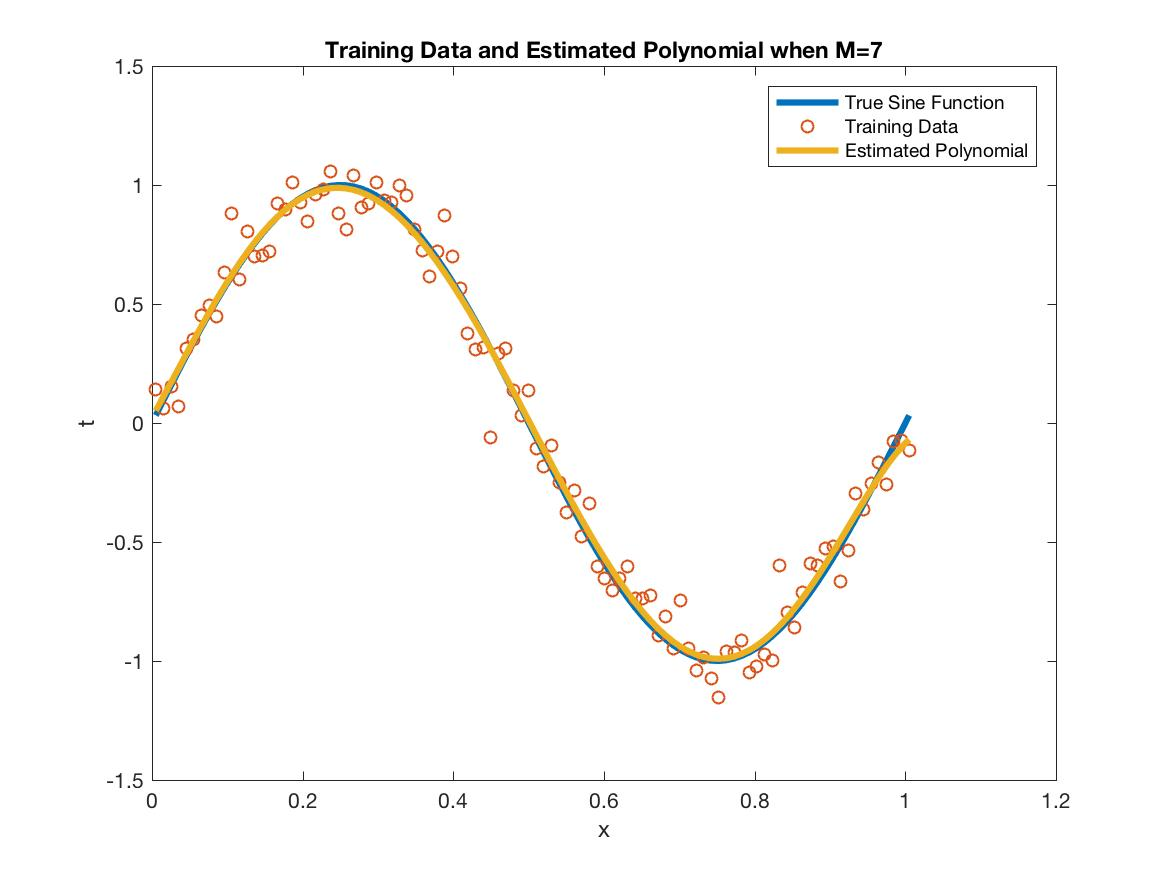
\includegraphics[width=3.4in]{7train.jpeg}
	        \caption{Training: M = 7}
	        \label{fig:side:a}
	    \end{minipage}%
	  \begin{minipage}[t]{0.5\textwidth}
	      \centering
	      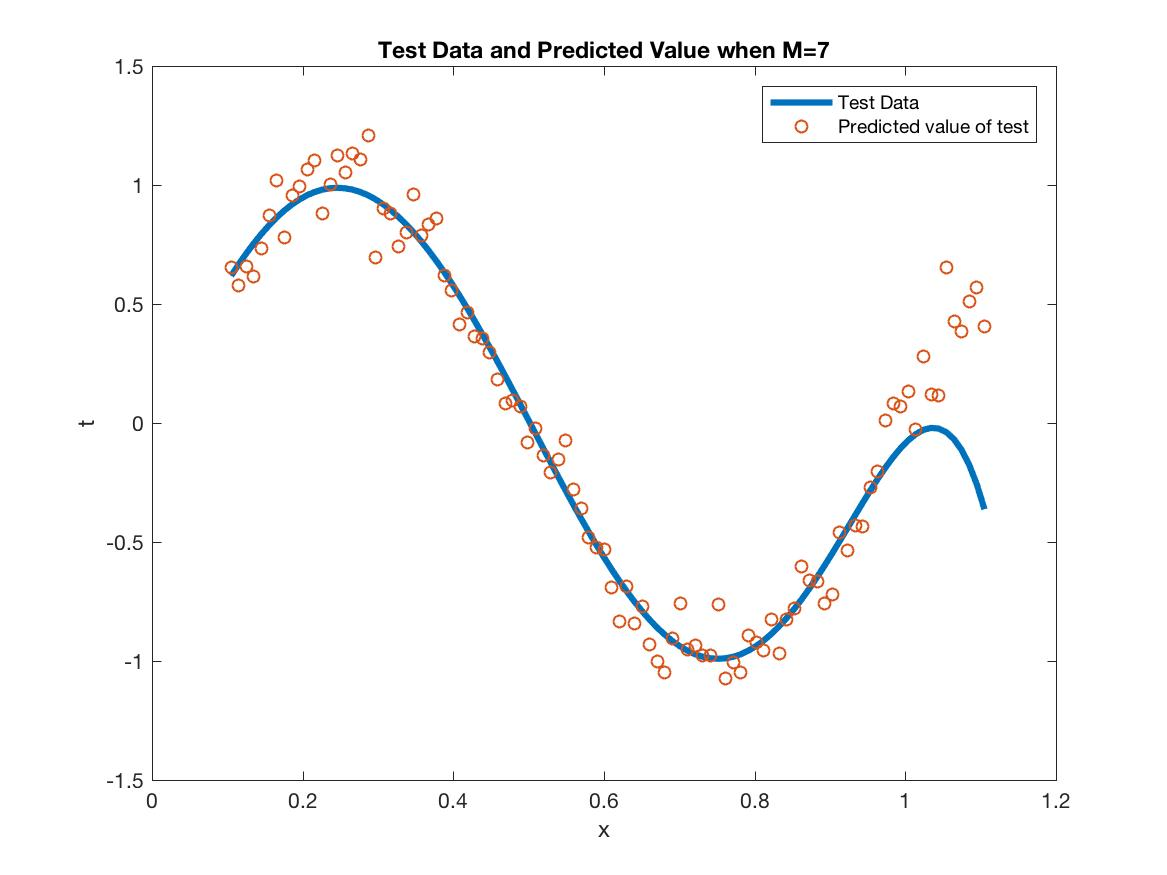
\includegraphics[width=3.4in]{7test.jpeg}
	      \caption{Test: M = 7}
	      \label{fig:side:b}
	    \end{minipage}
	\end{figure}

	\begin{figure}[H]
	    \begin{minipage}[t]{0.5\textwidth}
	        \centering
	        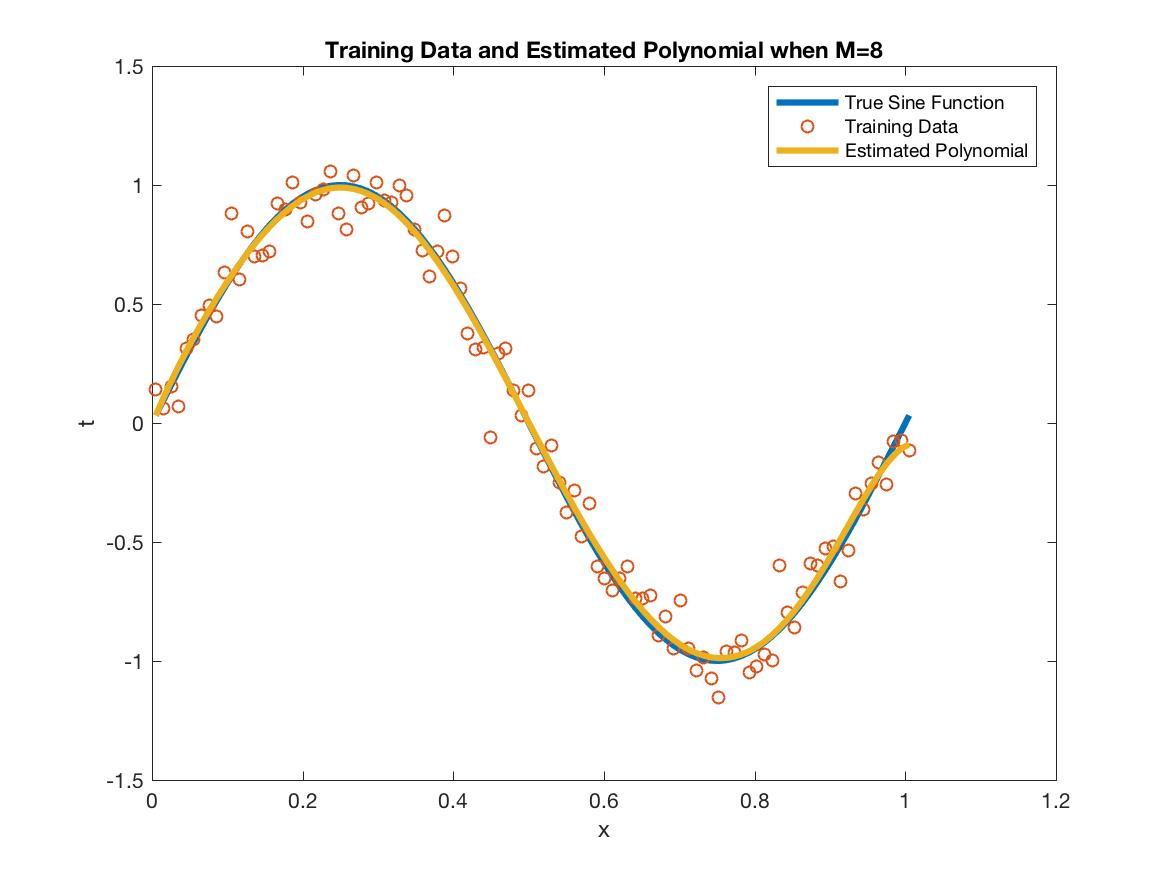
\includegraphics[width=3.4in]{8train.jpeg}
	        \caption{Training: M = 8}
	        \label{fig:side:a}
	    \end{minipage}%
	  \begin{minipage}[t]{0.5\textwidth}
	      \centering
	      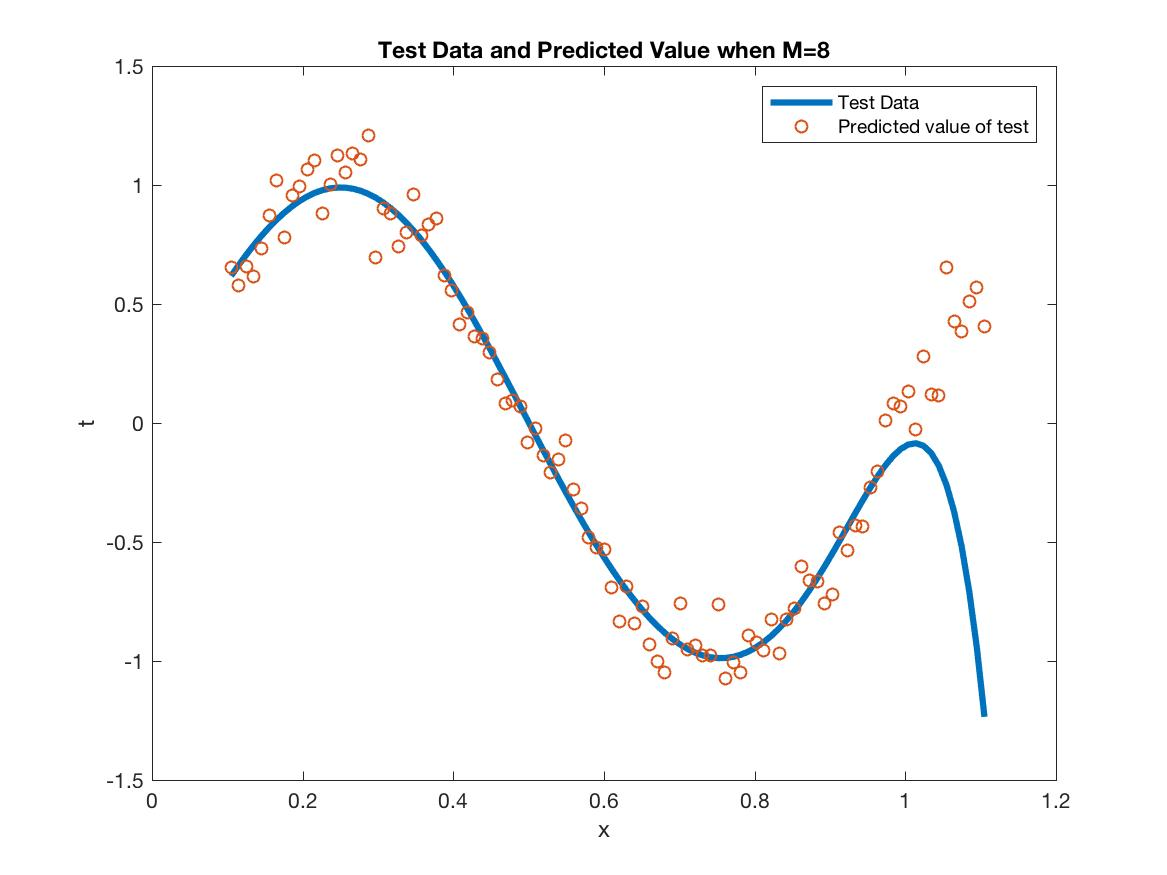
\includegraphics[width=3.4in]{8test.jpeg}
	      \caption{Test: M = 8}
	      \label{fig:side:b}
	    \end{minipage}
	\end{figure}	
		
	\begin{figure}[H]
	    \begin{minipage}[t]{0.5\textwidth}
	        \centering
	        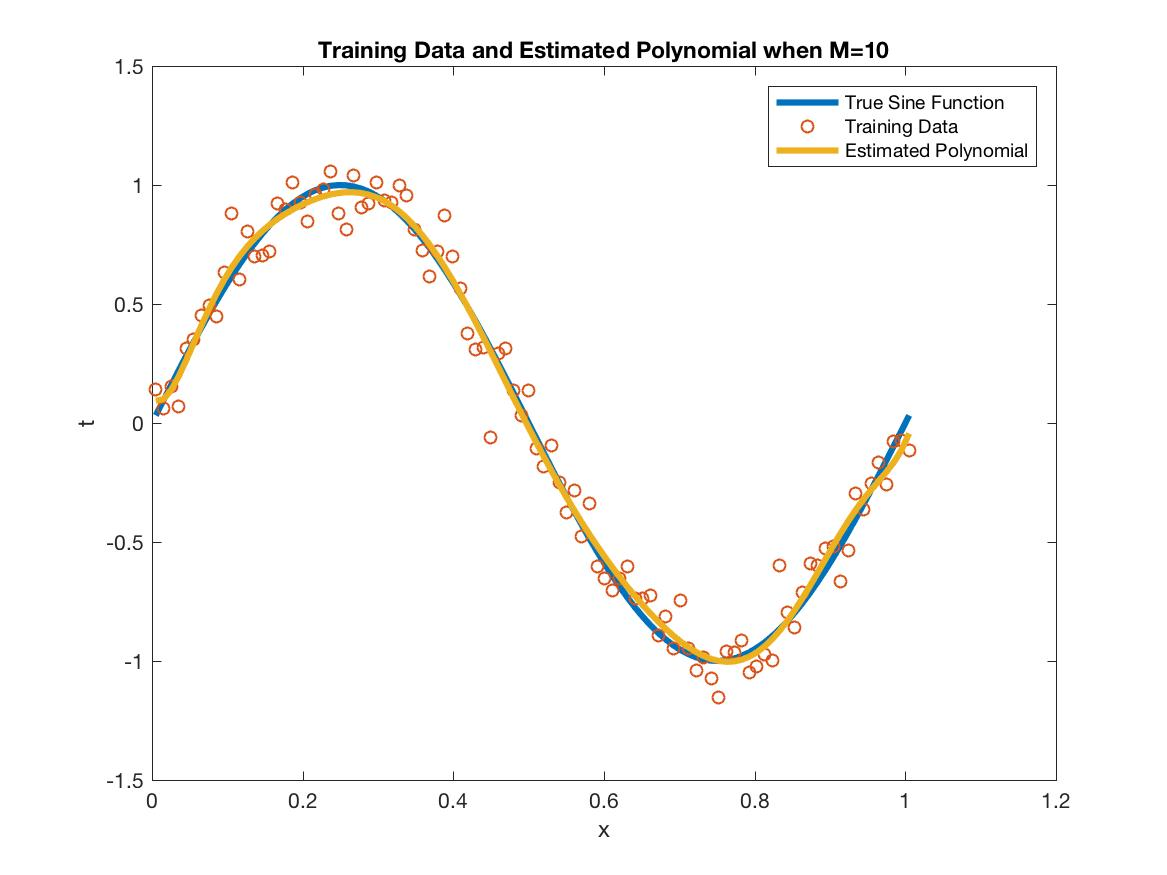
\includegraphics[width=3.4in]{10train.jpeg}
	        \caption{Training: M = 10}
	        \label{fig:side:a}
	    \end{minipage}%
	  \begin{minipage}[t]{0.5\textwidth}
	      \centering
	      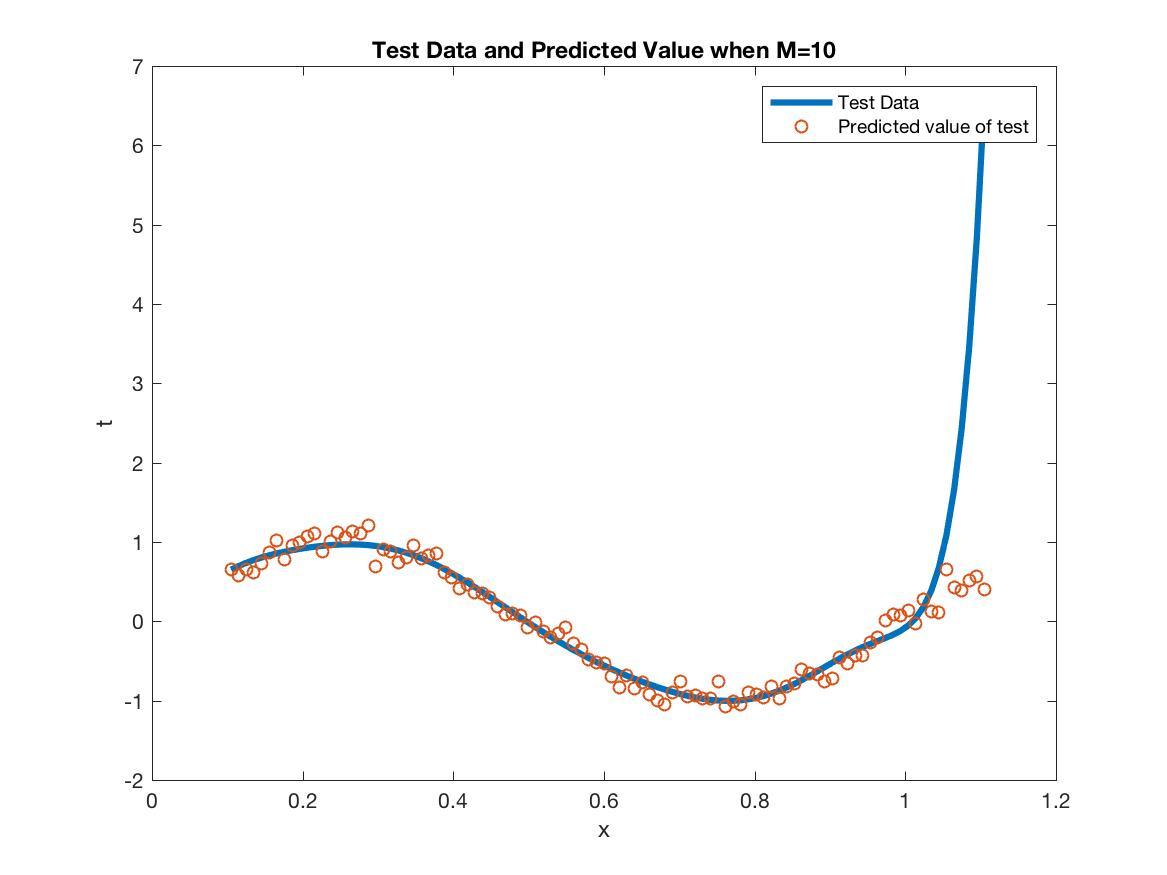
\includegraphics[width=3.4in]{10test.jpeg}
	      \caption{Test: M = 10}
	      \label{fig:side:b}
	    \end{minipage}
	\end{figure}

	Actually, as the the model order M increases, it is intuitively by the graphs that the polynomial fits the training data 	better, while it fits the test data poorer every time. As it can also told through the graphs of the $E_{RMS}$ 		evaluating for both training set and test set (Figure 15). RMS(root-mean-square) error is defined by: $E_{RMS} = 	\sqrt{2E(\boldsymbol{w})/N}$. If the model order is too small, say, $M \leq 2$, the polynomial curve fitting has the 	problem of underfitting, i.e., the model is unable to capture the underlying trend of the data. While if the model is 	quite large, the polynomial curve fitting has the problem of overfitting, i.e., the model fits the training set nearly 		perfect, but it is too complex and it has poor predictive performance for the test set(e.g. Figure 11, 12, 13 and 14).\\
	Based on the results I got, I would say using model order $M = 5$ to get minimum of both training and test RMS error. 
	
	\begin{figure}[H]
	    \centering
	    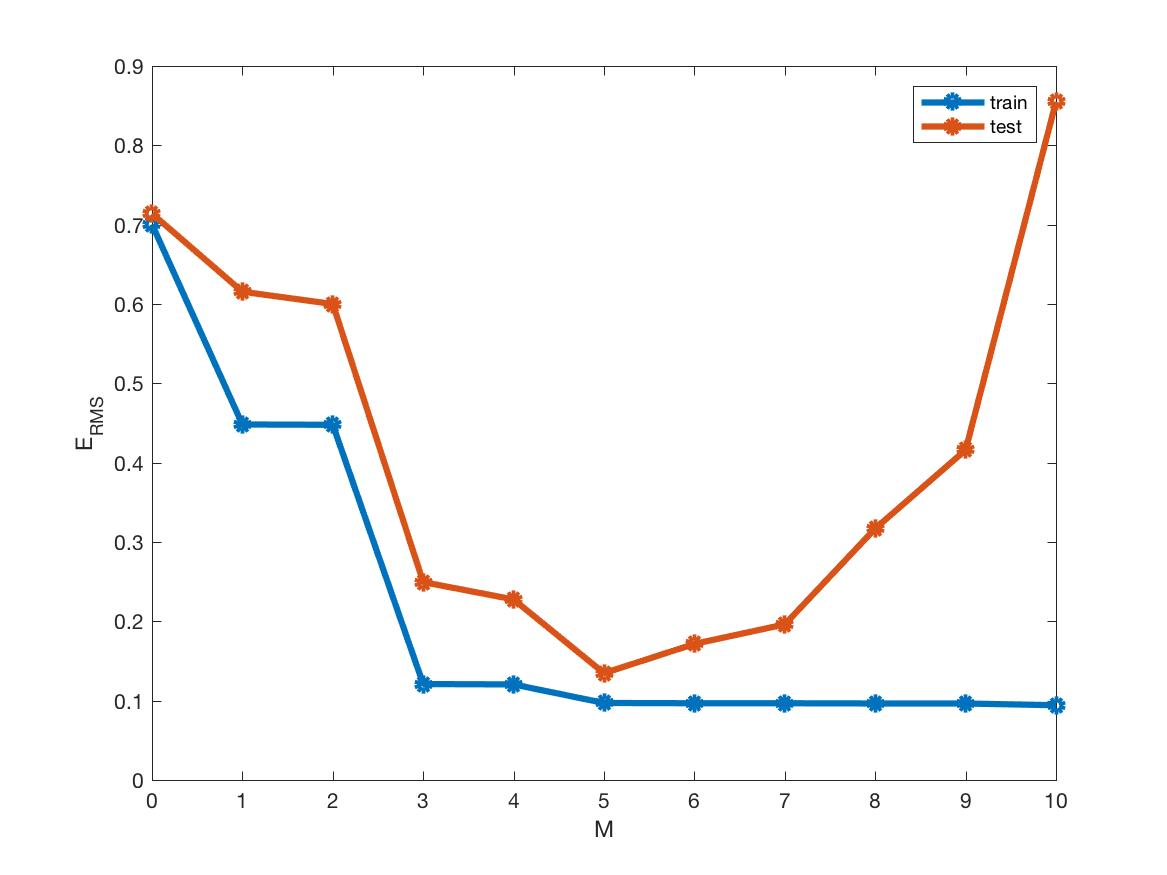
\includegraphics[width=6in]{ERMS.jpeg}
	    \caption{Graphs of the root-mean-square error evaluating for both training set and test set for various values of M}
	\end{figure}

	
\huge{\textbf{ Question 2}}      \Large{Solution:} \\
	\normalsize 
	Based on the known sizes of matrices or vectors: $\bf{X}$: $M \times N$, \ \  $\bf{Y}$: $N \times N$, \ \  $\bf{a}$: $M
	\times 1$, \ \  $\bf{b}$: $N \times 1$\\
	We got the sizes of corresponding transposes: $\bf{X^T}$: $N \times M$, \ \  $\bf{Y^T}$: $N \times N$, \ \  $\bf{a^T}
	$: $1
	\times M$, \ \  $\bf{b^T}$: $1 \times N$.\\
	And $s$ is a scalar.
	\begin{enumerate}
		\item The operation $\bf{XY}$ is defined. The size of the resulting answer is $M \times N$.
		\item The operation $\bf{YX}$ is undefined.
		\item The operation $\bf{YX^T}$ is defined. The size of the resulting answer is $N \times M$.
		\item The operation $\bf{aX}$ is undefined.
		\item The operation $\bf{a^TX}$ is defined. The size of the resulting answer is $1 \times N$.
		\item The operation $\bf{aX^T}$ is undefined.
		\item The operation $\bf{a^Tb}$ is undefined.
		\item The operation $\bf{b^Tb}$ is defined. The resulting answer is a scalar.
		\item The operation $\bf{bb^T}$ is defined. The size of the resulting answer is $N \times N$.
		\item The operation $s\bf{X+Y}$ is undefined.\\
	\end{enumerate}

\huge\textbf{ Question 3}      \Large{Solution:} \\
	\normalsize 
	$\because$ $rank(X) = r$, $\therefore$ $rank(X^H) = r$, $\therefore$ $rank(XX^H) = rank(X^HX) = r$. While if $XX^H$ has the size $l\times l$, $X^HX$ may have the size $n\times n$ ($XX^H$ and $X^HX$ do not have to have the same size).\\
	Suppose $XX^H$ has the eigenvalue $\lambda$ and the eigenvector $\bf{u}$, we got $XX^H\bf{u} = \lambda\bf{u}$. \\
	If we multiply $X^H$ to the left of both sides of the above equation, we got: $X^HXX^H\bf{u}$ $= X^H\lambda\bf{u}$.\\
	Which is equivalent to $(X^HX)X^H\bf{u}$ $= \lambda X^H\bf{u}$. Thus we can conclude that $X^HX$ and $XX^H$ have the same eigenvalue $\lambda$. And if $XX^H$ has the eigenvector $\bf{u}$, $X^HX$ has the eigenvector $X^H\bf{u}$.\\

\huge\textbf{ Question 4}      \Large{Solution:} 
	\normalsize
	\begin{enumerate}
		\item $\displaystyle\frac{\partial f}{\partial \bf{x}} = 3(\displaystyle\frac{\partial \bf{x}^T\bf{x}}{\partial \bf{x}}) +
		4(\displaystyle\frac{\partial \boldsymbol{y}^T\boldsymbol{x}}{\partial \boldsymbol{x}}) - (\displaystyle\frac{\partial 1}{\partial \boldsymbol{x}}) = 3(\boldsymbol{x} + (\boldsymbol{x}^T)^T) + 4((\boldsymbol{y}^T)^T) + 0 = 6\boldsymbol{x} + 4\boldsymbol{y}$.
		
		\item $\displaystyle\frac{\partial^{2} f}{\partial \boldsymbol{x}^2} = \displaystyle\frac{\partial (6\boldsymbol{x}+4\boldsymbol{y})}{\partial \boldsymbol{x}} = \boldsymbol 6 = 6\boldsymbol{I}$, $\boldsymbol{I}$ is the identity matrix.\\
	\end{enumerate}


\huge\textbf{ Question 5}      \Large{Solution:} 
	\normalsize
	\begin{enumerate}
		\item $\displaystyle\frac{\partial f}{\partial \bf{x}} = -10[\bf{Qx} + (\bf{x}^T\bf{Q})^T] + (4\bf{y}^T)^T = -10[\bf{Qx} 
		+ \bf{Q}^T\bf{x}] + 4\bf{y}$.\\
			$\because$ $\bf{Q}$ is a symmetric matrix,\\
			$\therefore$ $\bf{Q^T} = \bf{Q}$.\\
			$\therefore$ $\displaystyle\frac{\partial f}{\partial x} = -20\boldsymbol{Qx} + 4\boldsymbol{y}$.\\
			
		\item $\displaystyle\frac{\partial^{2} f}{\partial \boldsymbol{x}^2} = \displaystyle\frac{\partial (-20\boldsymbol{Qx} + 4\boldsymbol{y})}{\partial 
		\boldsymbol{x}} = -20\boldsymbol{Q}^T = -20\boldsymbol{Q}$.\\
	\end{enumerate} 

\end{spacing}
\end{document}